\documentclass{article}
\usepackage{tikz}
\usetikzlibrary{arrows.meta}

\begin{document}

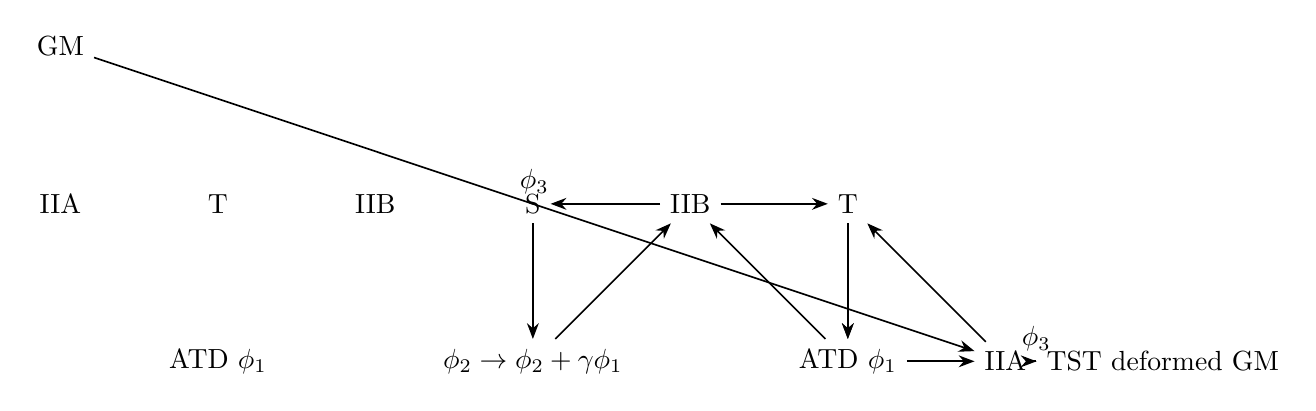
\begin{tikzpicture}[->,>=Stealth,shorten >=0pt,auto,node distance=2cm, semithick]
    \node (GM) {GM};
    \node[below of=GM] (IIA) {IIA};
    \node[right of=IIA] (T) {T};
    \node[below of=T] (ATD) {ATD $\phi_1$};
    \node[right of=T] (IIB) {IIB};
    \node[right of=IIB] (S) {S};
    \node[below of=S] (phi2_to_phi2_plus_gamma_phi1) {$\phi_2 \to \phi_2 + \gamma\phi_1$};
    \node[right of=S] (IIB) {IIB};
    \node[right of=IIB] (T) {T};
    \node[below of=T] (ATD) {ATD $\phi_1$};
    \node[right of=ATD] (IIA) {IIA};
    \node[right of=IIA] (TST_deformed_GM) {TST deformed GM};

    \draw (GM) -- node[above] {$\phi_3$} (IIA);
    \draw (IIA) -- (T);
    \draw (T) -- (ATD);
    \draw (ATD) -- (IIB);
    \draw (IIB) -- (S);
    \draw (S) -- (phi2_to_phi2_plus_gamma_phi1);
    \draw (phi2_to_phi2_plus_gamma_phi1) -- (IIB);
    \draw (IIB) -- (T);
    \draw (T) -- (ATD);
    \draw (ATD) -- (IIA);
    \draw (IIA) -- node[above] {$\phi_3$} (TST_deformed_GM);
\end{tikzpicture}

\end{document}